%!TEX ROOT=../dissertation.tex

\chapter{ČTK Dataset Collection}
\label{chap:ctk}
In Chapter~\ref{chap:fever_cs}, we have acquired the initial fact-checking dataset in Czech via localizing that of~\cite{fever}. The localized dataset relies on the \textsf{Wikipedia} dump as its knowledge base.

As the \textsf{Wikipedia} does not call itself a reliable source for a multitude of reasons~\cite{wiki:reliable}, a further research is desirable on how to transfer the fact verification practice learned on \textsf{FEVER} to a whole other knowledge base.

This raises a variety of interesting challenges, in particular: how to transition away from the encyclop\ae{}dic style~\cite{wiki:style} of written language? Could one transfer the fact-checking rules learned on such a strictly formatted corpus to, say, an archive of {news reports}, with all of its pitfalls, such as the \textit{temporal reasoning}\footnote{Typical case would be a journal archive containing two mutually exclusive \textit{ground truths} different in their timestamps, s. a. \"{Summer 2018 was the warmest} and \"{Summer 2019 was the warmest}}?

\section{Academic Cooperations}
As a part of the project \textit{\"{Transformation of Ethical Aspects With the Advent of Artificial Intelligence Journalism}} funded by the \textsf{Technology Agency of the Czech Republic} (\textsf{TAČR}), we have been given an opportunity to work with Václav Moravec from the \textsf{Faculty of Social Sciences}, \textsf{Charles University} (\textsf{FSS}), and the students of his courses in \textit{AI Journalism}.

Furthermore, we have been granted access to the full archive of \textsf{Czech News Agency} (\textsf{ČTK}), that, by the time of creating a snapshot, contained a total of 15,032,152 news reports released between $1^{st}$ January 2000 and $6^{th}$~March~2019\footnote{Efforts are being made to re-insantiate the following data collection experiments on an extended version of the archive, up to December 2020, so as to cover the topic of COVID-19 pandemic. These were, however, postponed subsequent to this thesis, in order to maintain its data consistency.}, which we have reduced to the size of 11,134,727 reports by removing the sport results and daily news summaries.

Thanks to these cooperations, we have been offered to work with around 170 human annotators, mostly undergraduate and graduate students of \textsf{FSS}. During three \"{waves} of annotation, we have collected a total of 10,084 data points (3,293 original claims and their respective labels and evidence).

In this chapter, we would like to describe how we tailored our own annotation platform to the needs of our task and annotators, justify the design choices that we made, and summarize our experience of supervising three waves of human claim generation and labeling experiment.


\section{Requirements for the Annotation Platform}
\label{sec:requirements}
Before we unravel the solutions provided by our platform, let us first spend a section to establish the underlying problems. Even though we do not follow any strict procedure of the \textit{requirements modelling}~\cite{requirements}, we believe that what follows are the most important challenges our system should tackle and other researchers building such a tool might want to keep in mind:

\begin{enumerate}
    \item {\techbf FEVER-like annotation tasks} -- despite the corpus differences, we aim to follow the concept-proven task division from~\cite{fever}:
    \begin{enumerate}
        \item[\itembox{\textsf{WF1a}}] \textbf{Claim Extraction} provides annotator $A$ with a document $d$ from the \textsf{Wiki} corpus, $A$ outputs a simple factoid claim $c$ extracted from $d$ without using $A$'s own world knowledge
        \label{wf1a}
        \item [\itembox{\textsf{WF1b}}]\textbf{Claim Mutation}: feeds $c$ back to $A$, who outputs a set of mutations of $c$: \\
        $M^c=\{m^c_1,\dots m^c_n\}$ using $A$'s own world knowledge (\textit{negation},~\textit{generalization},~\dots).
        
        For the completeness, we reprint the Table~\ref{fig:mutations} that lists the allowed types of mutations.\label{wf1b}
        
        %--- FIG: UTF forms
\begin{table}[H]
\begin{ctucolortab}
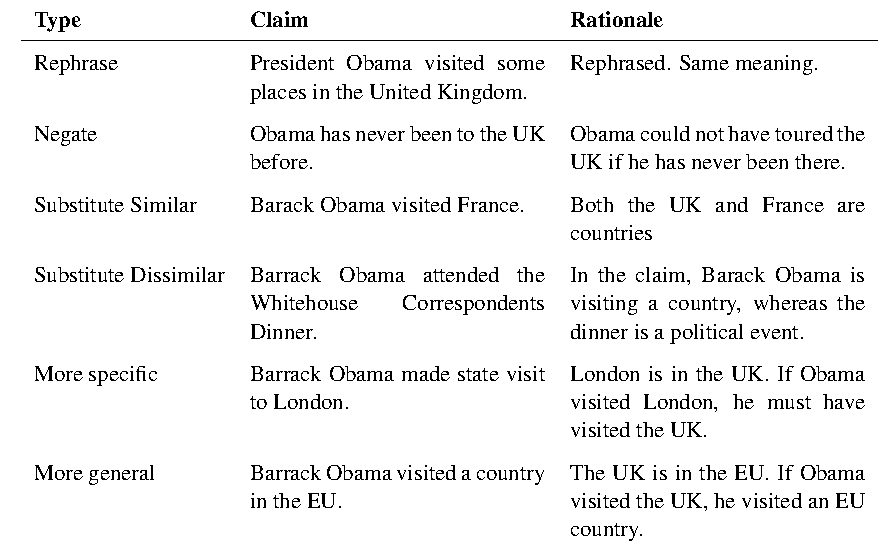
\includegraphics[width=12cm]{fig/mutations.pdf}
\caption[\textsf{FEVER Annotation Platform} mutation types]{\textsf{FEVER Annotation Platform} mutation types -- the examples mutate the claim \"{Barack Obama toured the UK} -- reprinted from~\cite{fever}}
\label{fig:mutations}
\end{ctucolortab}
\end{table}
%--- /FIG
        \item[\itembox{\textsf{WF2~}}] \textbf{Claim Labeling}: $A$ is given a sample of a mutated claim $m^c$, context that was given to extract $c$ in (a.) and is tasked to output sets of evidence $E^{m^c}_1,\dots,E^{m^c}_n$ along with the veracity label $g(E^{m^c}_i,m^c)$ which should be the same for each $i$. 
        \label{wf2}
        
        Apart from the context of $c$, $A$ can fulltext search the entire \textsf{Wikipedia} for evidence, however, $A$ operates under constrained time.
    \end{enumerate}
    
    \item {\techbf Paragraph-level documents} -- the \textsf{FEVER} shared task proposed a \textit{two-level} retrieval model: first, a set of \textit{documents}, i.e., \textsf{Wiki} abstracts is retrieved, then these are fed to the \textit{sentence retrieval} system which retrieves the evidence on the level of sentences.
    
    This simply does not work for us -- firstly, the sentences of a news report corpus are significantly less \textit{self-contained} than those of encyclop\ae{}dia abstract, not supporting the \textit{sentence}-level of granularity. Secondly, the articles tend to be overly long for the Document Retrieval task. 
    
    We argue that the best approach for our data is the \textit{paragraph-wise} splitting and a single level of retrieval, with an option of grouping a set of paragraphs by their source article. From this point we refer to the \textsf{ČTK} paragraphs also as to the \textit{documents}.
    
    \item {\techbf Source document sampling system} -- in~\cite{fever}, every claim was extracted from some sentence sampled from a \textsf{Wikipedia} abstract. With news report archive, this does not work well, as the majority of \textsf{ČTK} paragraphs does not contain an information eligible for fact-checking.
    \item {\techbf Limited knowledge oracle access} -- in \textsf{FEVER} \textbf{Claim Extraction} as well as in the annotation experiment of~\cite{danish}, the annotator was provided with a \textsf{Wikipedia} abstract and a \textit{dictionary} composed of the abstracts of articles \textit{linked} in it. This was important to ensure that the annotators only incorporate their full world knowledge in a restricted number of well defined tasks, and limit themselves to the facts (dis-)provable using the corpus in the rest.
    
    As the \textsf{ČTK} corpus does not follow any rules for internal linking, this will be a major challenge to reproduce. 
    \item {\techbf Annotator performance measures} -- completion of the annotation tasks is going to count towards the completion of the \textsf{FSS} course. Therefore, the annotator's identity needs to be stored within the system, and a set of reasonable goals must be proposed to track the completion of student's duties. 
    
    Reaching the goals should take under 3 hours on average, which matches the share of the annotation assignment on the \textsf{ECTS} study load of the \textsf{FSS} course~\cite{ects}.
    
    \item {\techbf Cross-annotator validation} -- to measure the validity of the annotations, as well as that of our novel platform, a claim should be labeled more than once on average.
    
    This will allow us to quantify the inter-annotator agreement, as well as it increases the overall number of evidence sets per claim. We do not consider the task of enumerating \textit{every} possible evidence set from the \textsf{ČTK} corpus feasible, as the news archives are not limited in the number of duplicate information they store. However, the more the better.
    
    \item {\techbf ČTK Archive access mediation} -- Due to the size of the \textsf{ČTK} archive (\char`~11M reports with metadata) and our space constraints that do not allow a very generous indexing, we need a caching system that only stores the articles necessary for annotating the claims that are currently in the system. This reduces the lookup time and increases the maximum traffic load.
\end{enumerate}

\section{FCheck Platform}
In Figure~\ref{fig:er}, we model the basic structures of data our system is working with and their relations using the standard entity--relationship diagram~\cite{10.1145/320434.320440}.

In contrast with the simplicity of the structured \textsf{JSONL} annotation format shown in the Figure~\ref{list:fever}, our data model is rather complex. Our aim here is to exploit the properties of relational database to find annotation ambiguities and easily compute the annotator performance measures through \textsf{SQL} \textit{aggregations}

In addition, we introduce the automatically updated \textsf{UNIX} timestamps \texttt{created\_at} and \texttt{updated\_at} to every entity from~\ref{fig:er}, to be able to reconstruct the annotation timeline, as well as to generate a dashboard of {live} visualisations of the performance and validity metrics, examples of which are the Figure~\ref{fig:crossannotations} and~\ref{fig:performance}.

\subsection{Entities and Their Relations}

Every annotator is to be identified through their respective \db{User} object, storing the neccessary credentials and signing every annotated data-point with their identifier. The data-points are divided into \db{Claim}s and \db{Label}s. Each \db{Claim} is either extracted from a \textsf{ČTK} \db{Paragraph}, linked as \texttt{paragraph}, or from a parent \db{Claim}, linked as \texttt{mutated\_from}.

\begin{figure}[H]

 \makebox[\textwidth][c]{{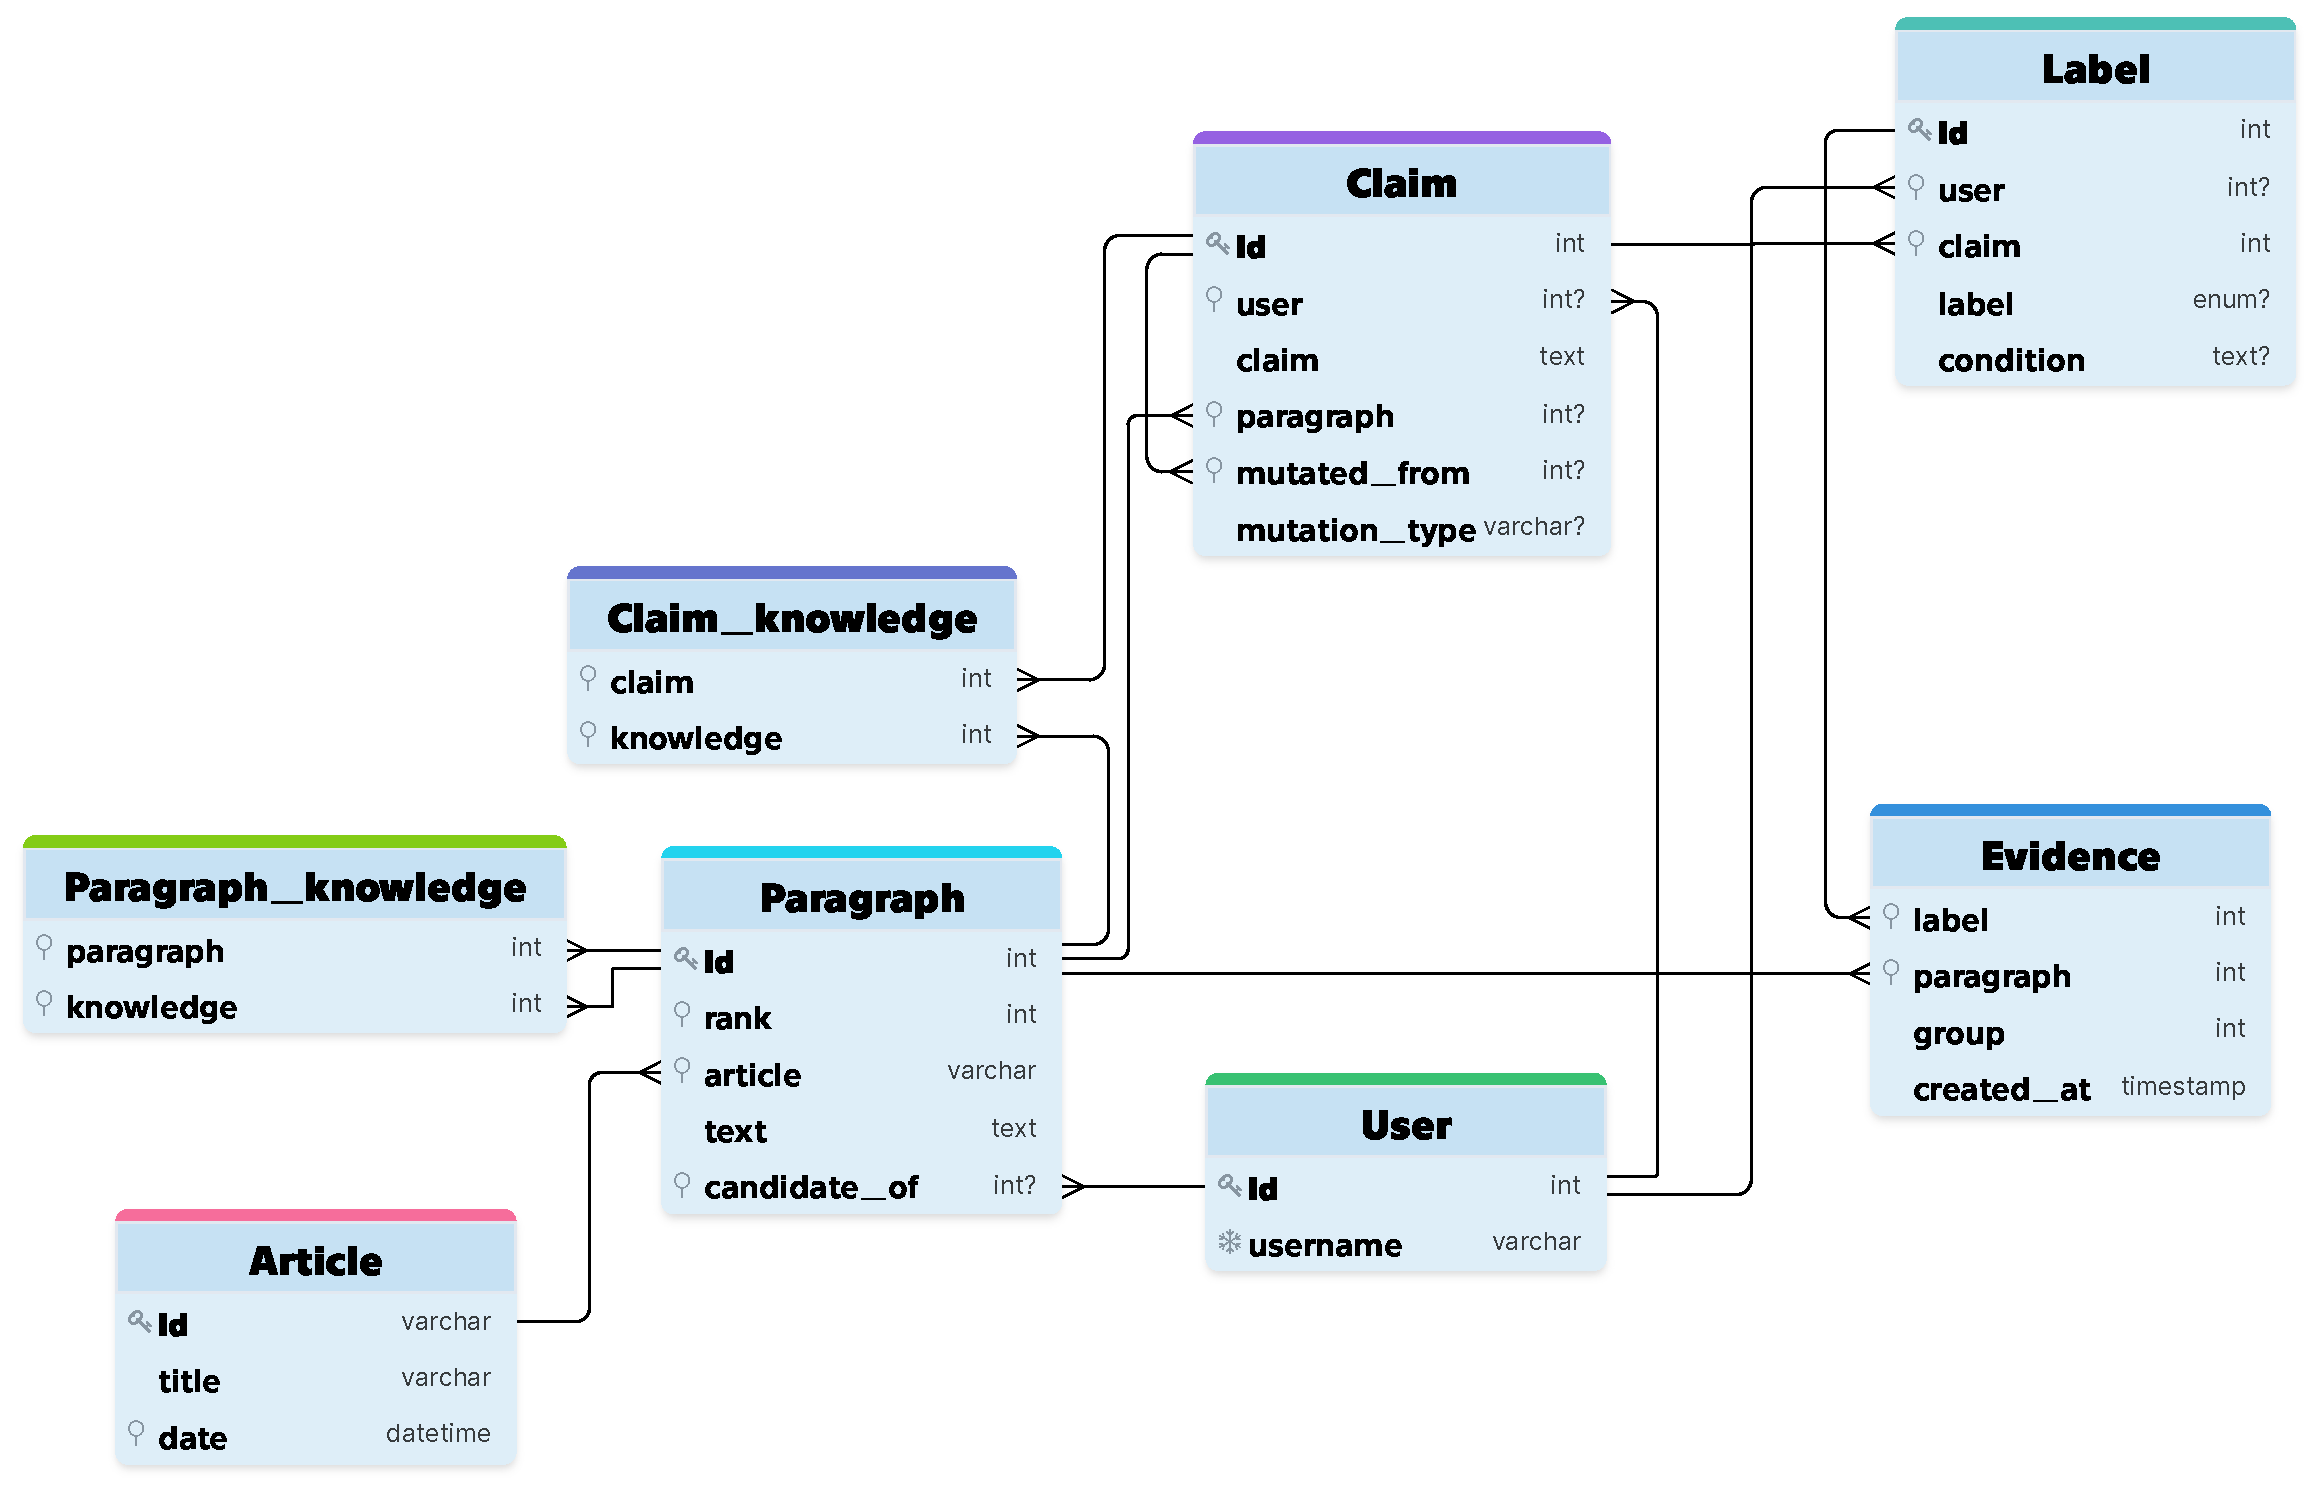
\includegraphics[width=18cm]{fig/er-diagram.pdf}}}

\caption{Entity--relationship diagram of the {\textsf{FCheck}} application drawn using \cite{drawsql}}
\label{fig:er}
\end{figure}%ER diagram

For the Claim Labeling and Claim Extraction tasks, user is to be given a restricted scope of knowledge. This knowledge can be described as a set of \db{Paragraph} objects, and is defined for a given \db{Claim} or \db{Paragraph} (\textit{many-to-many} relations \db{Paragraph\_knowledge} and \db{Claim\_knowledge}) -- we will define the \textit{knowledge scopes} in~\ref{sec:knowledge-scopes}.

The \db{Label} data-point is characterized by the \texttt{label} itself (\texttt{\textit{enum}} of \texttt{SUPPORTS},\texttt{REFUTES},\texttt{NOT ENOUGH INFO}) and its \db{Evidence} -- a set of \textit{evidence sets}. Each such evidence set consists of \db{Paragraph}s and is distinguished by a different ordinal number \texttt{group} stored alongside the \db{Evidence} relation. Therefore, a single \db{Label} can have multiple alternate sets of evidence, just as demonstrated in the Figure~\ref{list:fever}. 

Several complementary entities were hidden away for the simplicity of the~\ref{fig:er}, however, are not integral to the data model of our application -- for example the \textit{annotation stopwatch} data.

\subsection{Technology Stack}
Originally, we have planned to re-use the \textsf{Flask} annotation platform of~\cite{fever} with minor tweaks. Sadly, we were unable to fully recover the open source version\footnote{\url{https://github.com/awslabs/fever/tree/master/fever-annotations-platform}}, as there was static data of unknown structure missing for \textsf{Wiki} \textit{redirects}.

Even so, these efforts would have been rendered futile by the invention of \textit{knowledge scopes} that we will introduce in~\ref{sec:knowledge-scopes}.

Thus, we have embarked on the journey to build our very own annotation platform, heavily inspired by that of~\cite{fever}, using our preferred technologies:

\begin{enumerate}
    \item {\techbf PHP 7} will be running the annotation back-end, written using the {\techbf Yii2} framework, served by {\techbf Apache2} on {\techbf Debian} 
    \item {\techbf MySQL 8} is to be storing the entities from~\ref{fig:er} in form of the \textsf{SQL} tables
    \item {\techbf Python 3.7}, {\techbf PyTorch}, {\techbf Flask} and {\techbf SQLite3} provide an \textsf{API} for a direct {\textsf{ČTK}} data access, as well as to the neural networks and clustering required for semantic search
    \item {\techbf AJAX} will be used to asynchronize the \textsf{API} calls, so that a user can keep annotating on the \textsf{Apache} server while the computation-heavy tasks are being processed by \textsf{Flask}
\end{enumerate}
Despite the choice of technologies does not follow the most recent trends, we have decided for it because of its familiarity. As the annotation leadership and administration are tasks heavy on technical support and hotfixing, we favoured the tools we have several years of commercial experience with.


\subsection{Corpus Caching: Proxy Entities}
\label{sec:proxies}
The \db{Article} and \db{Paragraph} \textsf{db} entities from~\ref{fig:er} serve as a proxy for the slowly attainable entries of the full \textsf{ČTK} corpus which is stored separately and its paragraphs are copied to the \textsf{FCheck} database on demand.

The idea is that if we provide a background service that asynchronously precomputes which paragraphs of the full corpus are to be provided to an annotator for the given task and input data, we can simply copy them into a well-indexed smaller database integrated with the rest of the system through a relational database. 

Thus, we were able to scale down the amount of data hardwired to the interactive part of the platform from \char`~$10^8$ to the order of $10^4$ paragraphs, dramatically improving the lookup times while also obtaining a compact \textit{self-contained}  database that can be easily backed up and still contain all the corpus entries necessary for exporting the dataset.


\subsection{Knowledge Scopes}
\label{sec:knowledge-scopes}
\textit{In place of \textsf{Wikipedia} \textit{dictionaries} that were used used in \textsf{FEVER} annotation task, we propose the following framework for knowledge delimitation:}



We have used the \textsf{DrQA}~\cite{drqa} and \textsf{multilingual BERT}~\cite{devlin2019bert} models trained by~\cite{michal} during his summer \textsf{AIC} internship as our internal state-of-the-art for \textsf{FEVER CS} \textsf{wiki-}abstract retrieval. The model task was to output a set of $k$ semantically nearest paragraphs ($k$-NN) to the given string.

Where \textsf{DrQA} operates on a verbatim (\textit{term frequency–inverse document frequency}) basis, \textsf{mBERT} model calculates the paragraph \textit{embeddings} using a Transformer network pre-trained on \textsf{Wikipedia} and finetuned for the Czech Document Retrieval task.

To have the best of both worlds, we have used a simple \textsf{ČTK Archive Flask API}, implemented by~\cite{honzagit} as a \textit{façade} that receives a claim (or a paragraph identifier) through a \textsf{HTTP} request, and responds with a combination of the results of both of the aforementioned models.

\subsubsection{ČTK Archive Flask API}
Is a simple \textsf{HTTP API} we have co-authored with our supervisor Jan Drchal. It encapsulates the access to the \textsf{ČTK Archive} corpus via \textit{random sampling} and the \textit{Knowledge scope} enumeration, which follows:

In brief words, it makes multiple calls to the \textsf{DrQA}, fortifying the claim by a different pair of mentioned \textit{named entities} in each\footnote{E. g. the claim \"{Miloš Zeman visited Slovakia.} is augmented by an extra copy of the entity \"{Miloš Zeman}, and \"{Slovakia}, to boost their \textit{term frequency}.}, to obtain their highest-utility results for each NE pair. Then it picks the 4 documents with the \textit{overall} highest utility as the \texttt{search\_ner} result. The Named Entity Recognition is handled by the model of~\cite{strakova-etal-2019-neural}.

It then retrieves the 1024 top documents for the query using \textsf{mBERT}, and clusters their embeddings into 2 groups with $k$-means. Then, two closest representatives of the \textit{claim embedding} from every cluster are stored as the \texttt{search\_semantic}.

The flask ouputs both \texttt{search\_ner} and \texttt{search\_semantic}, i.e., a maximum of 8 documents per query, not to overwhelm the annotator. Furthermore, it makes sure that all the retrieved paragraphs have an older timestamp than the input. This outlines our solution for the \textit{temporal reasoning} issue. Simply put, to each claim, we assign a date of its formulation, and only verify it using the news reports published \textit{to that date}.

Using the example from the~\hyperref[chap:ctk]{chapter introduction}, the paragraph \"{Summer 2019 was the warmest} (say, published at Septamber $24^{th}$, 2019) will only be considered a \textit{ground truth} for claims with a timestamp $\geq \texttt{2019-09-24}$. For the completeness, later, in the task \tjednab{}, we assign each claim with the publication timestamp of its source paragraph.

\section{The Annotation Workflow}
In the previous sections, we have explained the technical challenges and their respective solutions. An equally important task is that of supervising a group of annotators new to this system and streamlining a sequence of tasks that both guides the annotators to the best use of their expertise in journalism and saturates the dataset.



\subsection{Revised Annotation Tasks}


To satisfy our requirements, we have adjusted the annotation tasks from Section~\ref{sec:requirements} in the following ways: 

\textit{For reader's convenience, we mostly use a simplified set of actors -- \textsf{Flask} is the \"{slow} back-end \textsf{API}, that operates above with the full \textsf{ČTK Archive} and models from~\ref{sec:knowledge-scopes}, \textsf{Apache} is a lighter web interface above the entities of~\ref{fig:er} accessible to $A$, $A$ is the annotator.}
\begin{enumerate}
        \item[\itembox{$\textsf{T}_{\textsf{0~}}$}] \textbf{Source Paragraph Preselection:} \textsf{Flask} samples a source article, \textsf{Apache} caches it (see~\ref{sec:proxies}). $A$ spends $~\leq 30$ seconds skimming the article and, finally, nominates a single paragraph $p$ to be used in $\textsf{T}_{\textsf{1a}}$. 
        
        $p$ must feature a \textit{self-contained} piece of verifiable information. If there is no such paragraph, $A$ skips to the next sample. 
        
        Otherwise, \textsf{Apache} stores the nomination and \textsf{Flask} enqueues the \textit{knowledge scope} computation for $p$. Once finished, result will be forwarded to \textsf{Apache}, which will cache the retrieved paragraphs and their respective articles and store them as $knowledge(p)$.
        
        
        \label{t0}
        \item[\itembox{$\textsf{T}_{\textsf{1a}}$}] \textbf{Claim Extraction:} \textsf{Apache} samples a nominated paragraph $p$, provides $A$ with $p$ and $knowledge(p)$. $A$ outputs a simple factoid claim $c$ extracted from $\{p\}\cup knowledge(p)$ without using $A$'s own world knowledge
        \label{t1a}
        \item [\itembox{$\textsf{T}_{\textsf{1b}}$}]\textbf{Claim Mutation}: \textsf{Apache} feeds $c$ back to $A$, who outputs a set of mutations of $c$: \\
        $M^c=\{m^c_1,\dots m^c_n\}$ using $A$'s own world knowledge (\textit{negation},~\textit{generalization},~\dots)\label{t1b}
        
        To catch up with the additional knowledge introduced by $A$, \textsf{Flask} enqueues the computation of $\{knowledge(m^c_1),\dots knowledge(m^c_n)\}$, and, once done, notifies \textsf{Apache} to store these, as well as to cache the incident paragraphs.
        \item[\itembox{$\textsf{T}_{\textsf{2a}}$}] \textbf{Own (Oracle) Claim Labeling}: \textsf{Apache} samples a fresh $m^c$ made by $A$, and provides its source paragraph $p$, its full original article, and a shuffled set of articles from $knowledge(m^c)\cup knowledge(p)$.
        
        $A$ spends $\leq 3$ minutes looking for the evidence sets  $E^{m^c}_1,\dots,E^{m^c}_n$ along with the veracity label $g(E^{m^c}_i,m^c)$. \textsf{Apache} saves them as an \textit{oracle annotation}.
        \label{t2a}
        
                \item[\itembox{$\textsf{T}_{\textsf{2b}}$}] \textbf{Others' Claim Labeling}: same as \tdvaa{} for $m^c$ made by \textit{other} annotator than $A$. Stored as \textit{regular annotation}.
        \label{t2b}
    
    \end{enumerate}

\subsection{Conditional annotations}
During our tests of the interface, a common problem with the annotation task \tdva{} using the \textsf{ČTK} corpus was that of \textit{assuming the knowledge}. Using the mutation types such as \textit{generalization}, one would often run into generating a claim containing a mutation not fully provable using a news archive.

For example, for a claim \"{Miloš Zeman did not visit an European country}, system~\ref{sec:knowledge-scopes} often retrieves relevant knowledge s. a. \"{Miloš Zeman visited Slovakia}. However, it barely ever retrieves the neccessary conclusive proof that \"{Slovakia is a European country}.

To address this issue, we are introducing the concept of \textit{conditional annotations}: if the annotator can not construct an exhaustive evidence set, but possesses knowledge that would \textit{conclude} the \textit{partial} set of evidence, he is asked to write it down in a form of \textit{textual claim} $c_{condition}$. Then, if any annotator could \texttt{SUPPORT} the $c_{condition}$ using a freshly computed $knowledge(c_{condition})$, it would also yield the paragraphs that would \textit{complete} the partial sets of the original evidence.

\label{sub:conditional}
\begin{figure}[H]

    \begin{ctucolortab}
    
    \fbox{\begin{minipage}{\textwidth}
        \textbf{Claim:} \"{The Killers performed in \textbf{the second day} of Rock for People 2007.}
        
        \textbf{Label: }\texttt{REFUTES}
        
        \textbf{Condition:} \"{The first and the second day of Rock for People had disjoint line-ups.}
    \end{minipage}}
    \end{ctucolortab}

    ~
    

    \textit{Evidence set \#1:}
    \begin{ctucolortab}
    
    \fbox{\begin{minipage}{\textwidth}
\begin{hangparas}{2em}{1}
            {\textbf{The first day of Rock for People culminated with the concert of The~Killers [July $4^{th}$ 2007]}} 
            
            \hspace{1.7em} Hradec Králové, 4th of July (ČTK) - Today, an hour before midnight at the Hradec Králové airport, American guitar band The Killers performed their concert, which was the climax of \textbf{the first day} of the festival. Above the mucisians' heads hanged a shining sign \"{Sam's Town}, which is the name of their second album that came out last year. The musicians came to introduce the songs from this album to the festival audience.
\end{hangparas}
    \end{minipage}}
    \end{ctucolortab}

    
    \caption[Example of a conditional label]{Example of a conditional label (translated from the \textsf{ČTK v2.1} dataset). See that if we are able to \texttt{SUPPORT} the \textbf{condition}, we can use the union of any of its evidence-sets together with the set \textit{\#1} to disprove the original claim. If not, the correct label is \texttt{NEI}.}
    \label{fig:conditional}
\end{figure}

\section{Web User Interface}
Finally, we are including a look into the client-side of the annotation platform we have presented to our annotators. 

In~\ref{sec:requirements}, we have estimated a maximum time of \textbf{3 hours} to complete the entire annotation workflow (\ref{fig:annotation}). Of these, we have dedicated the first \textbf{30 minutes} to a \textbf{video-tutorial}\footnote{\url{https://fcheck.fel.cvut.cz/site/tutorial} or \url{https://youtu.be/AcarF4Rxexc}}, which, despite its length, worked well\footnote{
After refining the tutorial and the supplementary lecture after the first wave of annotations, we have observed a significant decrease in the task procrastination (see Figure~\ref{fig:performance}), which may also have been caused by other factors. However, it had a good impact on the traffic spread, as well as on the quality of \tdva{} sampling (Figure~\ref{fig:crossannotations}).} in giving every annotator a full platform walkthrough and a hands-on example for every task.

Therefore, each student should spend only \textbf{2.5 hours} on our platform to reach all the annotation goals from Figure~\ref{fig:annotation}. This puts pressure on the design of the client-side, to be as easy to use as possible, while still supporting the sophisticated features, s. a. the \textit{conditional-} and \textit{multi-annotation}. In this chapter, we will show the web interface for the main tasks, and justify the design choices made.

To our readers, we also provide the link to the live\footnote{For as long as the \textsf{FEE CTU} keeps providing us with the computing power\dots} platform which can be found at \url{https://fcheck.fel.cvut.cz} and accessed by typing  \texttt{testuser} into the \"{\textsf{SIDOS} ID} field. Do not worry to play around, as all of the \texttt{testuser}'s annotations can be easily omitted from the exports.

\subsection{Claim Extraction}
We present our final \tjednaa{} interface in Figure~\ref{fig:annotation}. The layout is inspired by the work of~\cite{fever} and, by default, hides as much of the clutter away from the user as possible. Except for the article heading, timestamp and the source paragraph, all the information such as the \textit{knowledge base} is collapsed and only rendered on user's demand. 

During the first run, user is instructed to read through detailed {\btn{Instructions}} in a \textsf{Bootstrap} \textit{modal} window, that, for the rest of the time, stay hidden away again not to distract the annotator. Apart from these, we have only added a brief instruction to each the form field as a reminder.

Annotator reads the source article and, if it lacks a piece of information he wants to extract, looks for it in the expanded article or knowledge base entry. Extracted claims are to be typed into a \textsf{HTML} textarea and separated by the line break, which was the most intuitive method we experimented with. User is encouraged to \btn{Skip} any source paragraph that is hard to extract. 

Throughout the platform, we have ultimately decided not to display any \textit{stopwatch}-like interface not to stress out the user. However, there is a simple tracking \textsf{JavaScript} running in the background, storing time spent on each page. From this data, we have measured that, excluding the outliers ($\leq10s$, typically the \btn{Skip}ped annotations and $\geq 600s$, typically a browser tab left unattended), average time spent on this task is \textbf{2 minutes 16 seconds} and the median is \textbf{1 minute 16 seconds}.

After the first wave of annotation, we have augmented the interface with a triple of \textit{golden rules} to avoid repeating the most common mistakes. More on that in~\ref{sec:golden-rules}.



\subsection{Claim Mutation}
Follows the UI conventions set by the Claim Extraction. Mutation types follow those of the \textsf{FEVER Annotation Platform} (Table~\ref{fig:mutations}) and are distinguished by loud colors, to avoid mismatches. The mutation types will be a topic for further innovations in future, as our annotation experiments did not yield a label-balanced dataset. 

Excluding the outliers, the overall average time spent generating a batch of mutations was \textbf{3m 35s} (median \textbf{3m 15s}) with an average of \textbf{3.98} mutations generated per claim.

\pagebreak
\begin{figure}[H]
\thispagestyle{empty}
\vspace{-1.5cm}
\makebox[\textwidth][c]{{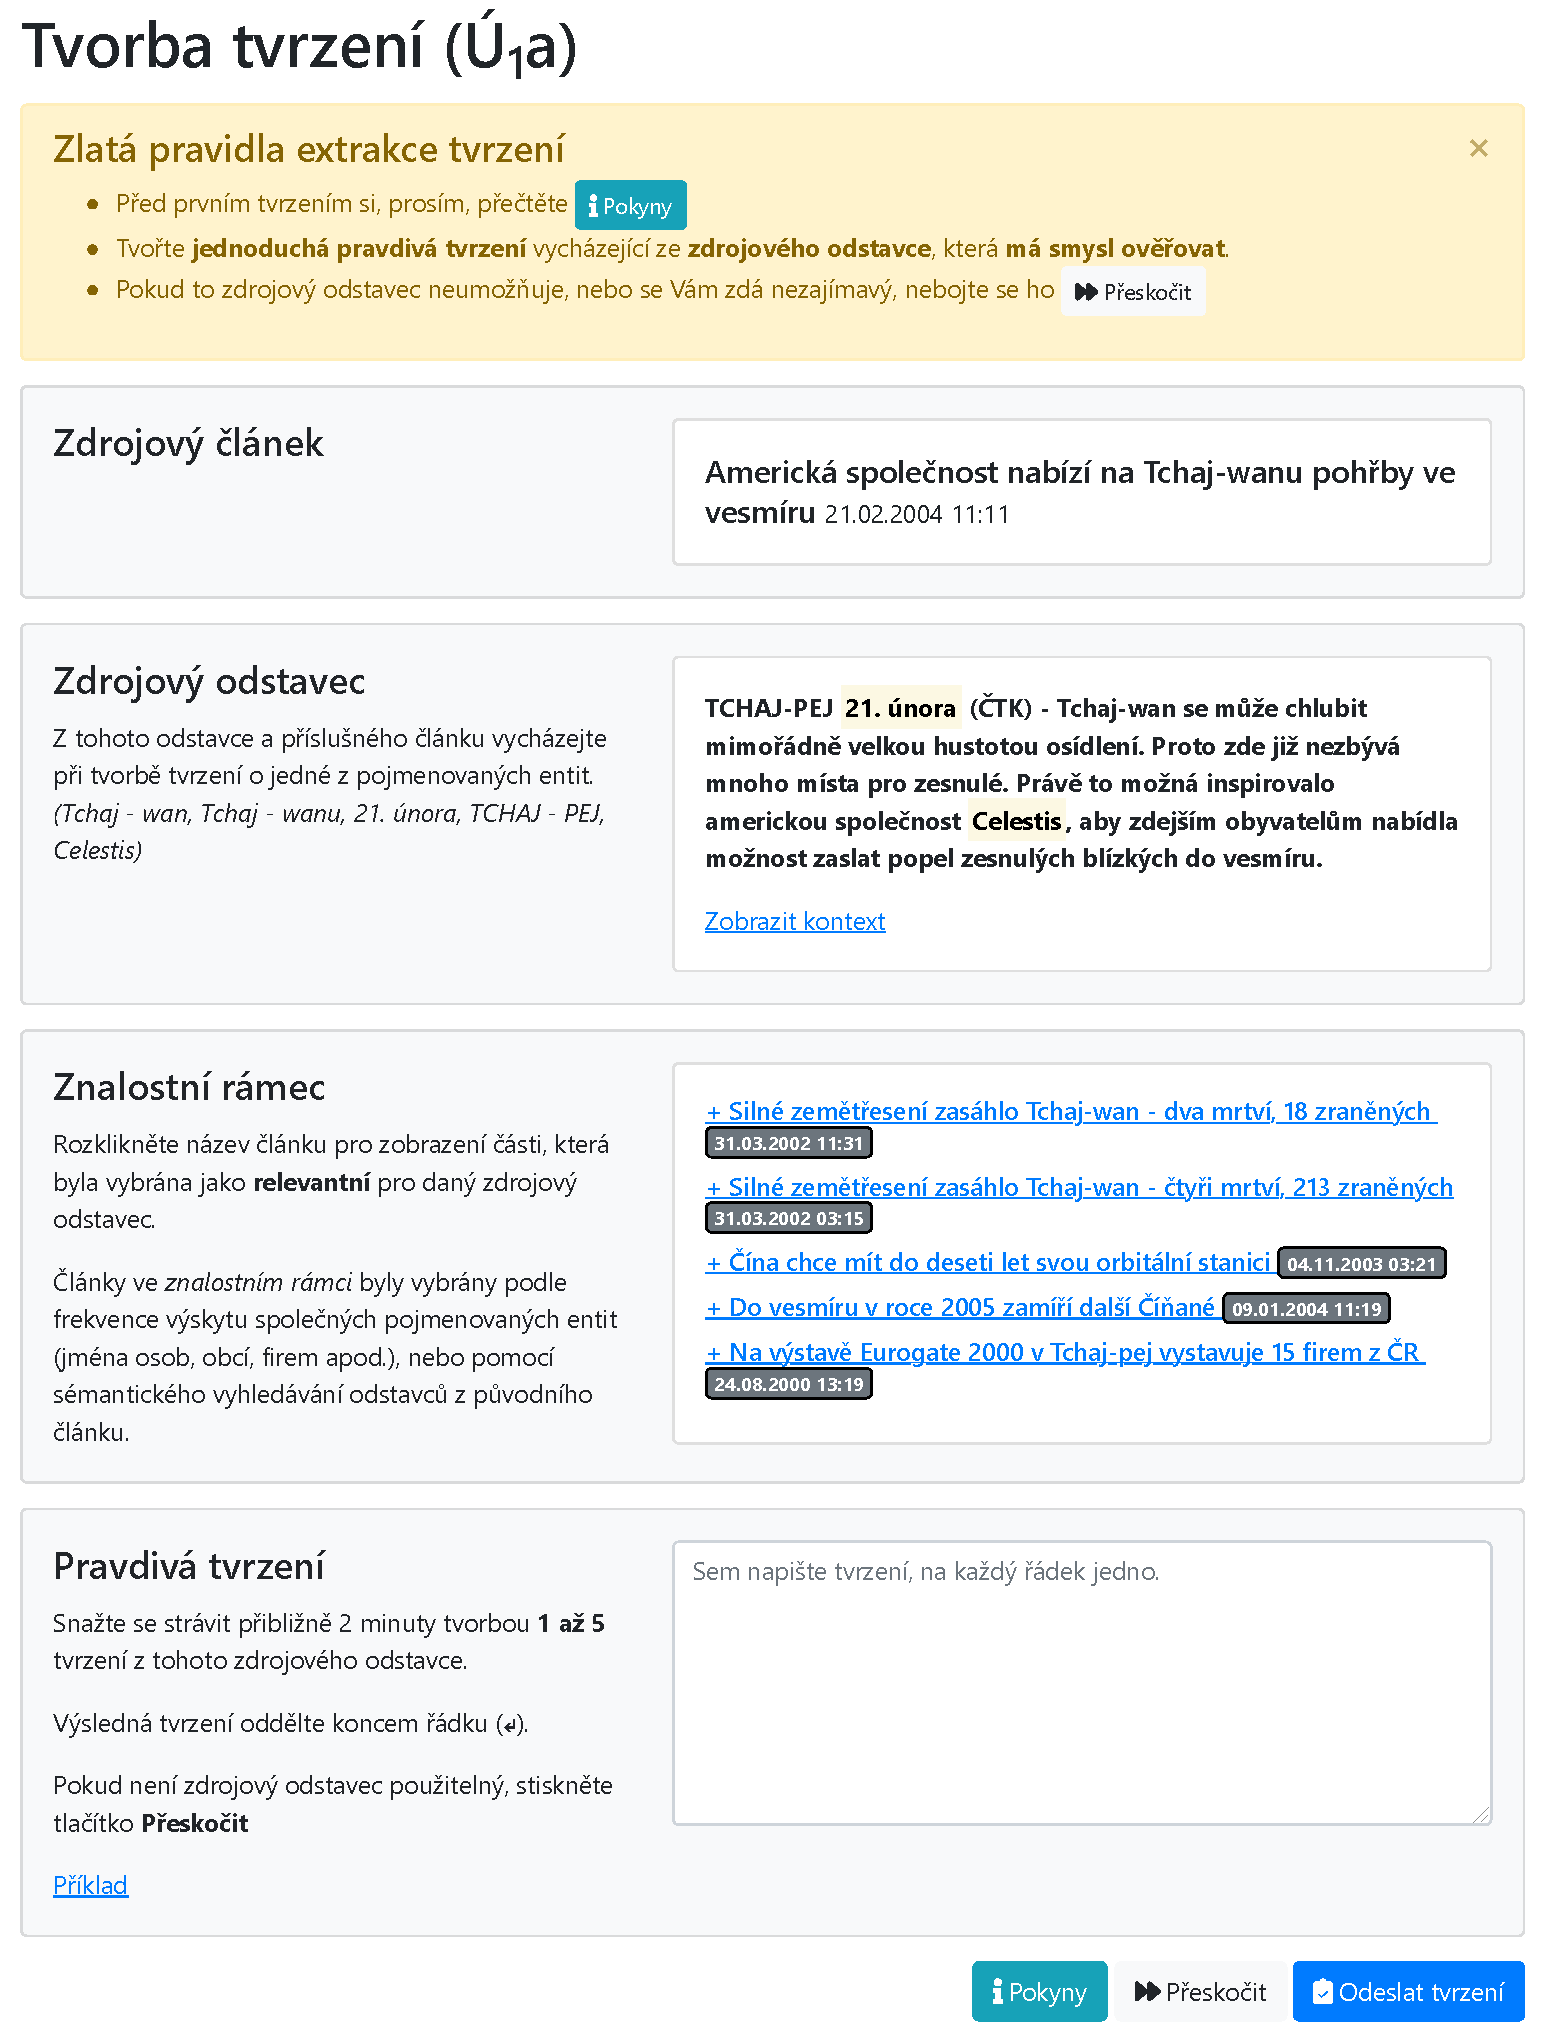
\includegraphics[width=19cm]{fig/claim_extraction.pdf}}}
\label{fig:extraction}
\caption[Claim extraction interface of \textsf{FCheck} platform]{Claim extraction interface of the \textsf{FCheck} platform}%Full English translation attached as Figure~\ref{trans:extraction} TODO: Friday
\end{figure} % Extraction
\pagebreak
\begin{figure}[H]
\thispagestyle{empty}
\vspace{-2cm}
 \makebox[\textwidth][c]{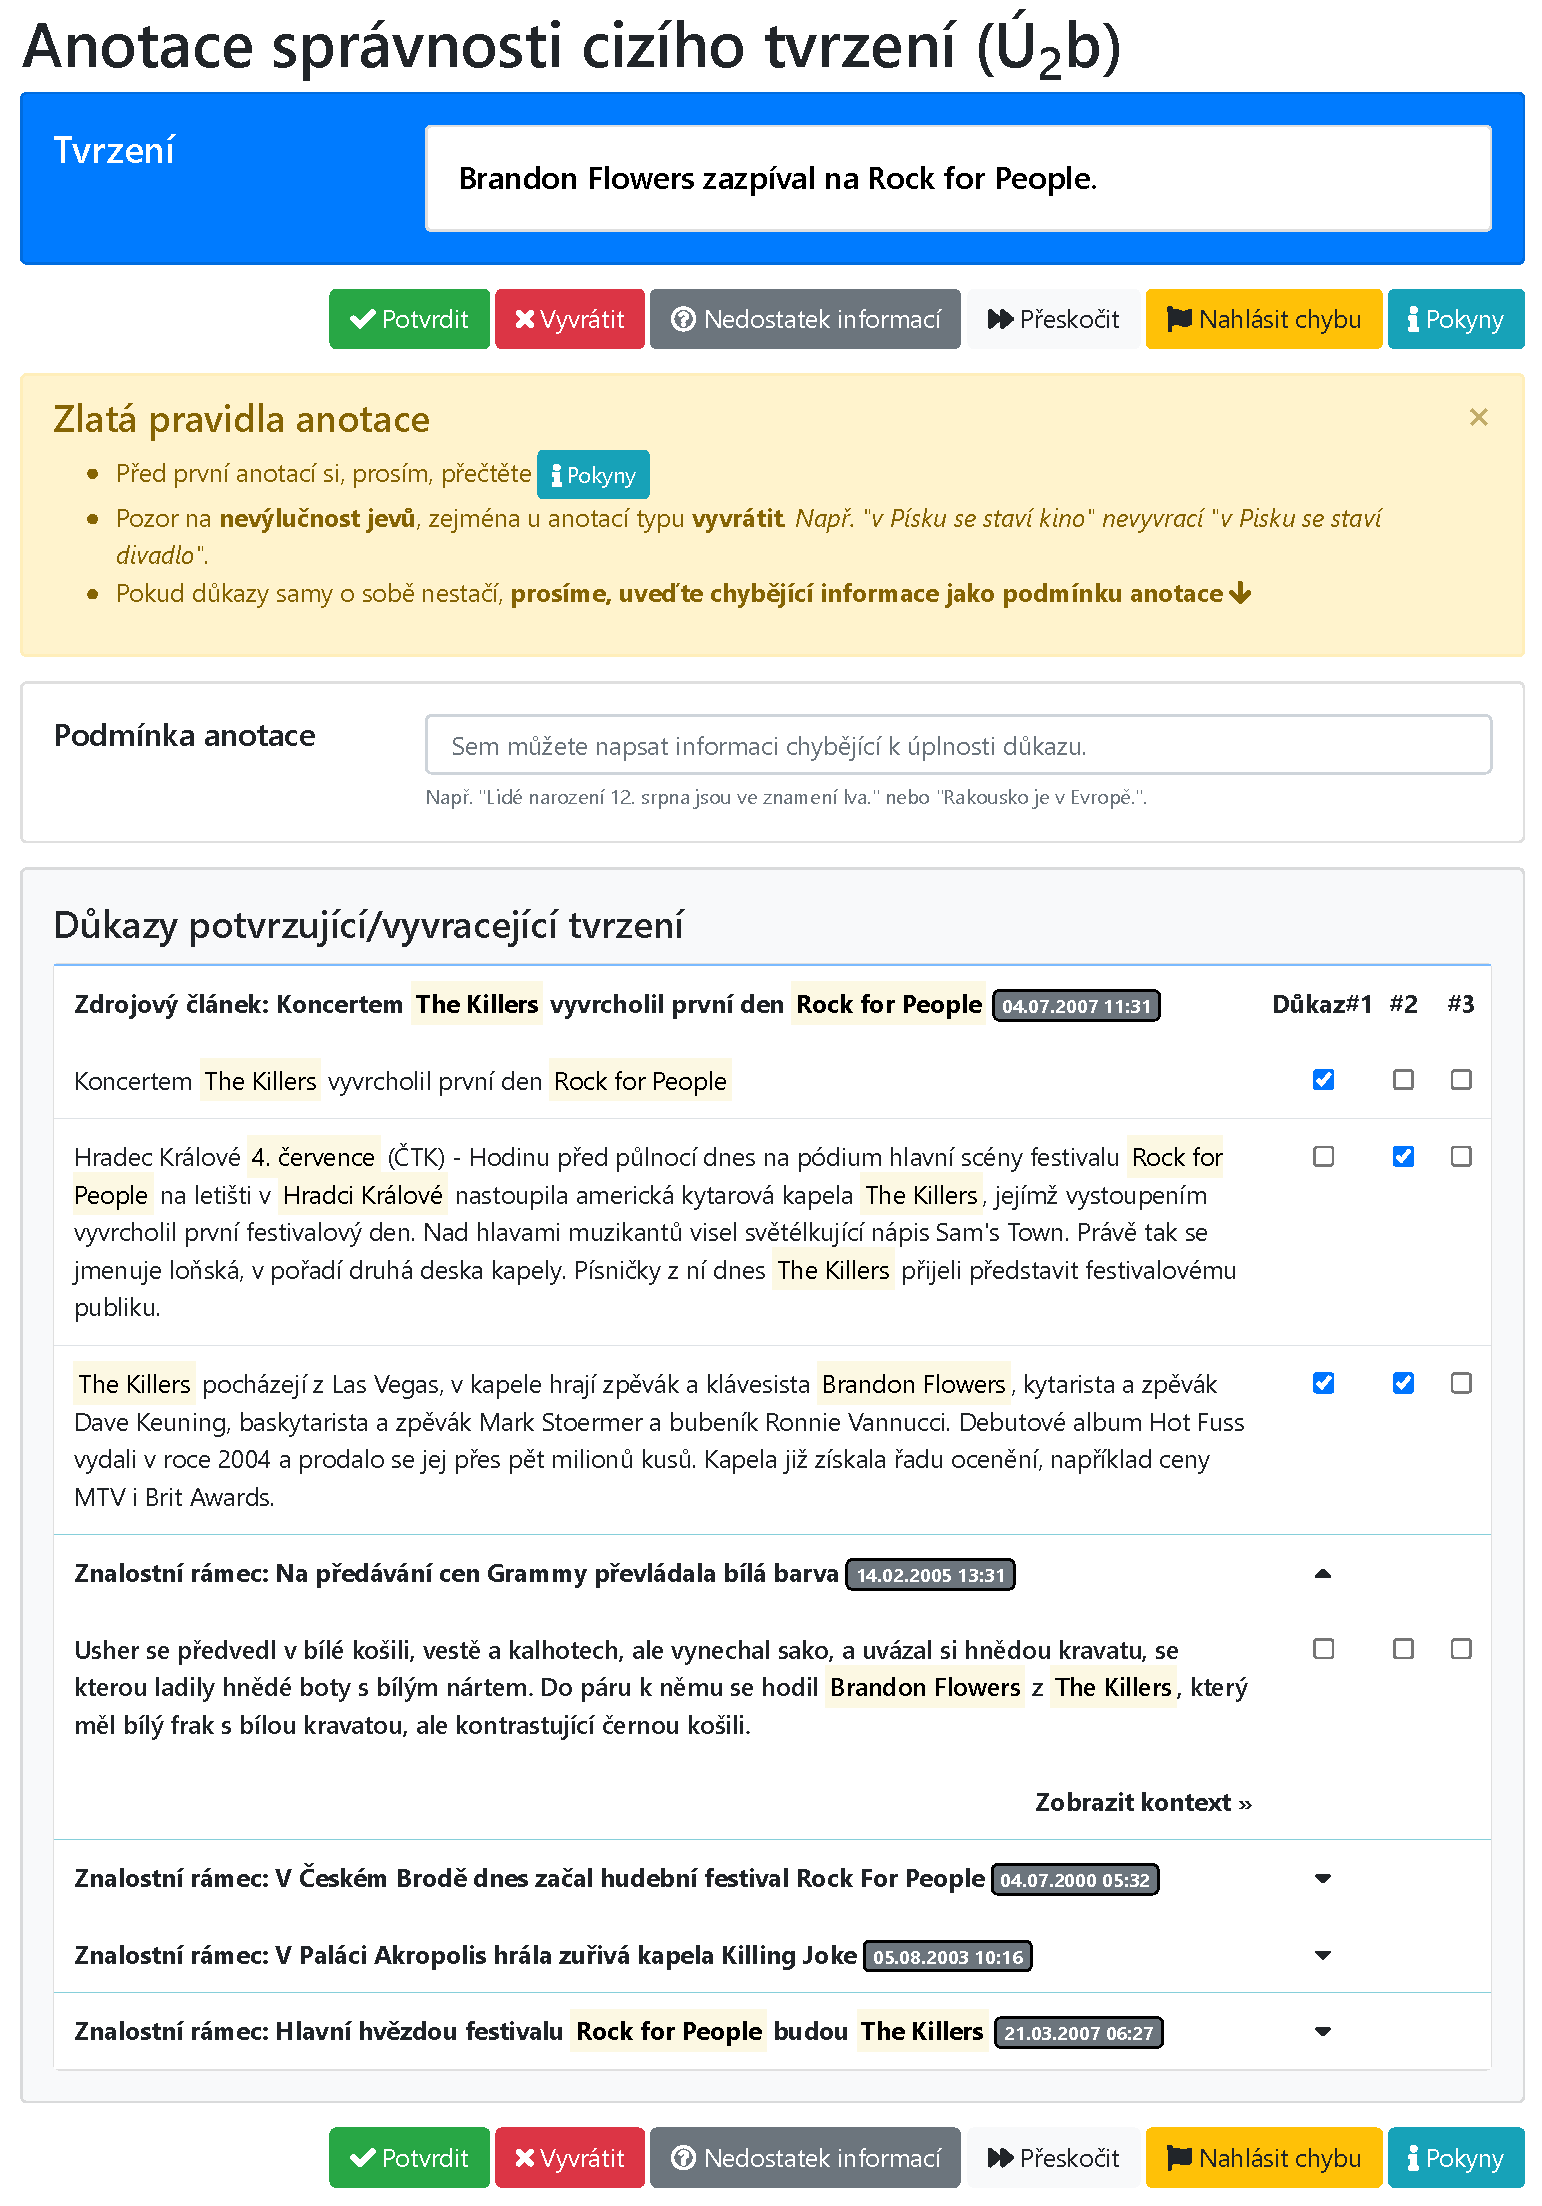
\includegraphics[width=18cm]{fig/annotation.pdf}}

\caption[Claim labelling interface of \textsf{FCheck} platform]{Claim labelling interface of \textsf{FCheck} platform. Full English translation attached as Figure~\ref{trans:annotation}}

\label{fig:annotation}
\end{figure} % Mutation
\pagebreak


\subsection{Claim Veracity Labeling}
\label{sec:ui-labeling}
In Figure~\ref{fig:annotation} we show the most complex interface of our platform -- the \tdva{}: \textbf{Claim Annotation} form. 

Full instructions take about 5 minutes to read and understand, and are hid away in the \btn{Instructions} modal window, that is to be opened during the first annotation, and the on demand. All actions are spread out on the top bar and \textit{label condition} is collected through a text field above the evidence input. This was decided after a negative experience with using a modal \btn{Actions} to hide away less frequent actions, originally inspired by other annotation platforms (see~\ref{sec:flat}).

The input of multiple evidence sets works as follows: each column of checkboxes in~\ref{fig:annotation} stands for a single evidence set, every paragraph from the union of knowledge belongs to this set iff its checkbox in the corresponding column is checked. Offered articles \& paragraphs are collapsible (without loss of checkbox state), empty evidence set is omitted. Through \textsf{JavaScript}, interface always displays all the non-empty sets defined so far, plus one empty column of checkboxes that can be used to initialize a new one.

On average, the labelling task took \textbf{65 seconds}, with a median of \textbf{40s}. An average \texttt{SUPPORTS}/\texttt{REFUTES} annotation was submitted along with \textbf{1.29} different evidence sets, 95\% of which were composed of a single paragraph -- full histograms will be introduced in Chapter~\ref{chap:dataset}.


\section{Between-Wave Platform Adjustments}
 \textit{\textit{Annotation wave} is our term for a group of \textsf{FSS} students annotating towards a common deadline, for a fixed period of 10--14 days.}
 
 \textit{To date, have supervised a total of a 4 annotation waves, however, as the wave 3 and 4 were largely simultaneous and their deadlines only differed in two days, we group them together as the \textit{$3^{rd}$ wave (Figure~\ref{fig:performance})}.}
 
  \begin{figure}[H]
\makebox[\textwidth][c]{{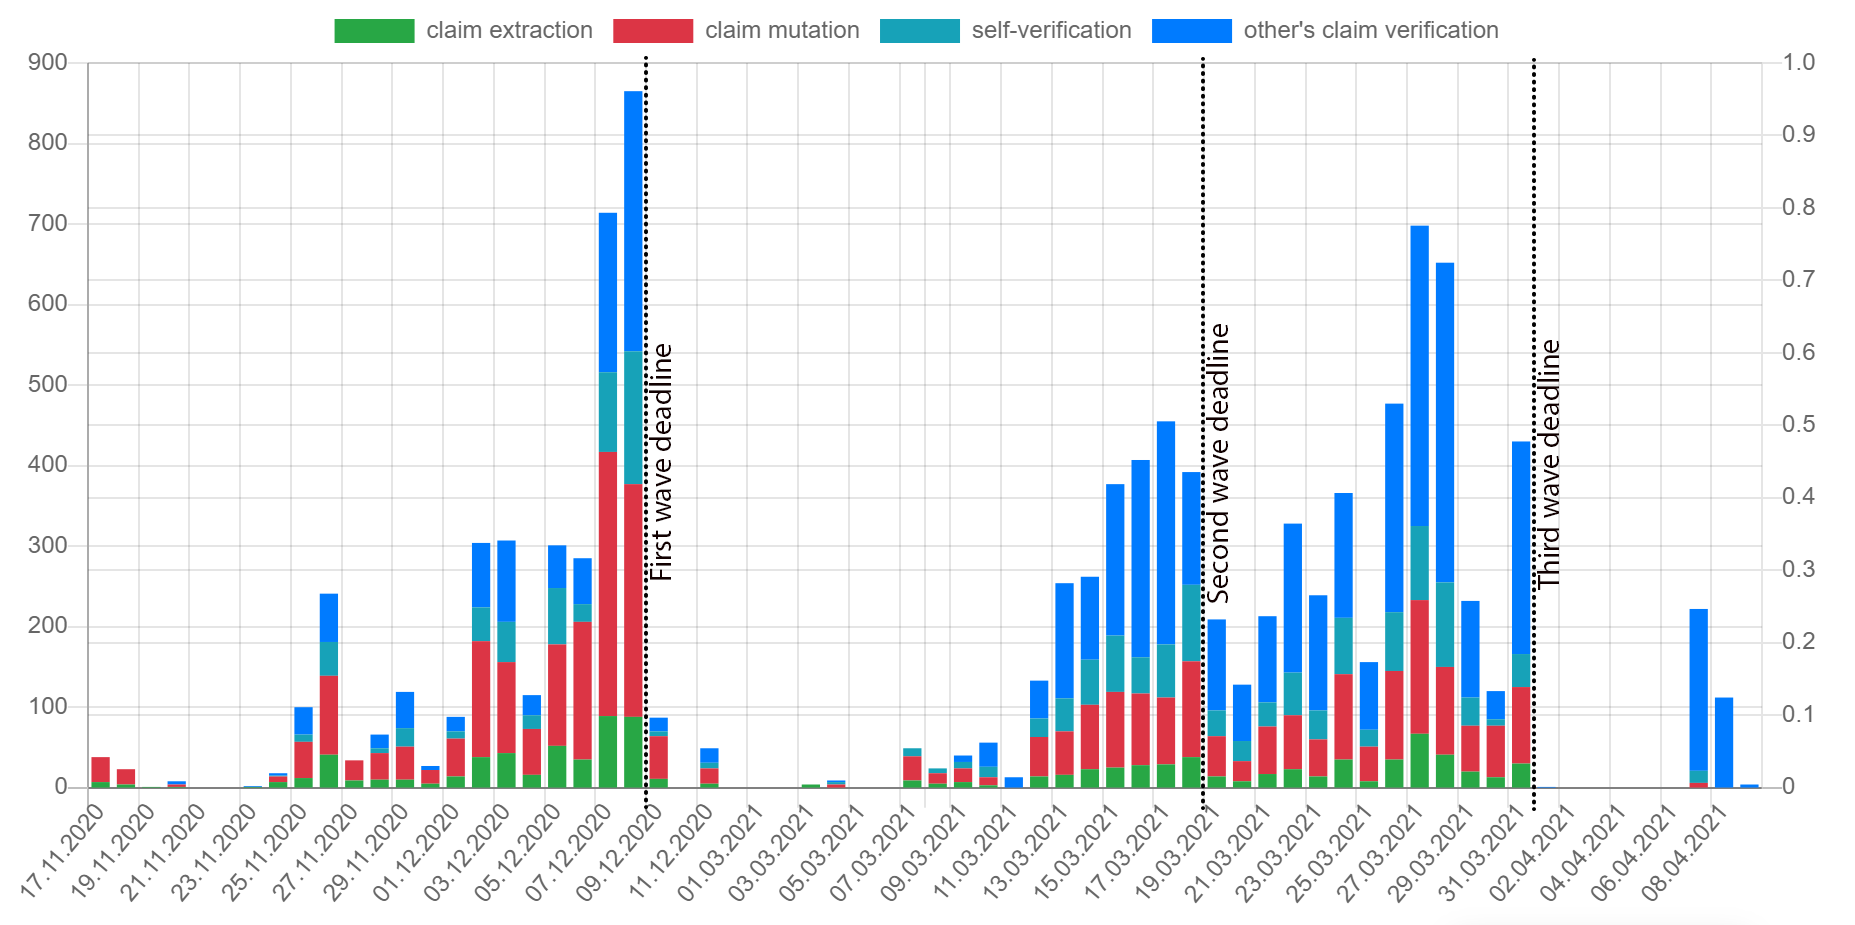
\includegraphics[width=18cm]{fig/performance.png}}}
\caption{Number of data points generated per day, colored by task}
\label{fig:performance}
\end{figure} % pestrobarevny graf
 
 Thanks to the multi-wave system of annotation, we were able to utilize our findings from the live data directly to patch the deployed version of the \textsf{FCheck} platform. This was particularly useful between the $1^{st}$ and the $2^{nd}$ wave. Here are the adjustments we presented, based on the learnings from the data exploration:


\subsection{The Golden Rules of Each Task}
\label{sec:golden-rules}
To address the most frequently reoccurring annotation errors, which will be examined in depth in Chapter~\ref{chap:dataset}, we have came up with a set of guidelines for each task. However, we found that the annotators tend to never re-read the full \btn{Instructions}, and to forget some of the important guidelines over time. Therefore, we have limited ourselves to 3 \textit{golden rules} per task, that will be present all the time, directly in the annotation task screen.


\begin{enumerate}
        \item[\itembox{\tjednaa{}}] \textbf{Golden Rules of the Claim Extraction:} 
        \begin{enumerate}
            \item[\itembox{1.}] Please read the \btn{Instructions} before making your first claim.
            \item[\itembox{2.}] Make \textbf{simple true claims} based on the source paragraph that\textbf{ make sense to be verified}.
            \item[\itembox{3.}] If the source paragraph doesn't allow that or seems uninteresting, feel free to \btn{Skip} it.
        \end{enumerate}
        \item[\itembox{\tjednab{}}] \textbf{Golden Rules of the  Claim Mutation:}
        \begin{enumerate}
            \item[\itembox{1.}] Please read the \btn{Instructions} before making your first mutation.
            \item[\itembox{2.}] {\techbf !} \textbf{Only make mutated claims that make sense to be verified.}
            \item[\itembox{3.}] Therefore, there is no need to use all 6 mutation types, 3 would suffice, even 1.
        \end{enumerate}
        \item[\itembox{\tdva{}}] \textbf{Golden rules of the Claim Annotation}: 
        \begin{enumerate}
            \item[\itembox{1.}]Before the first annotation, please, read the  \btn{Instructions}.
            \item[\itembox{2.}]Pay attention to \textbf{the non-exclusivity of phenomena}, especially for the \btn{Refute} annotations. \textit{E.g. \"{a cinema is being built in Písek} does not refute \"{a gallery is being built in Písek}}.
            \item[\itembox{3.}] If the evidence alone is not sufficient, please provide the missing information as a \textit{condition} of the annotation.
        \end{enumerate}
    \end{enumerate}
    
\subsection{T2: The Action Flattening}
\label{sec:flat}
After the first wave of annotation, that showed  a significantly underwhelming usage of \tdva{} actions grouped in an \btn{Actions} modal pop-up -- especially the usage of the \texttt{NOT ENOUGH INFO} label, \btn{Flag}s and \textit{conditions} -- we have re-thought the action toolbar and spread all the actions available onto a horizontal bar, each as a single button. If the action requires additional data, s. a. the \btn{Flag} reason, it only asks for it in a \"{next step} modal window.

\subsection{T2: User-Initiated Soft-Deletion}
\label{sec:soft-deletes}
In addition to this, we have added the feature of \textit{soft-deletes}. Thanks to the convenience of working with the \textsf{Yii2 PHP} Framework, we could simply constrain the system to only work with entity objects without the soft-deletion bit set to \texttt{1}, effectively augmenting each query above such an entity with \"{(\dots) \texttt{WHERE} (\dots) \texttt{AND deleted!=1}}.

Since the Wave 2, each \btn{Flag} was programmed to cause a temporary soft-delete of the flagged claim, to be re-considered by an administrator. This has shown to be a great synergy of the human-power of the annotators and admin's unconstrained system access. Admin got notified every time there was a claim containing a typo, a contradiction, or claim unrelated to the source paragraph, and did his best to fix the claim using his direct \textsf{db} access. In the meantime, the claim was inaccessible to the web user interface, and no annotation was wasted on invalid data. 

Over the waves 2 and 3, we have received a total of \textbf{112} flags, effectively saving almost \textbf{4 hours} of compromised annotation, estimated using the average \tdva{} load (\ref{sec:ui-labeling})  and 2 cross-annotations per claim. We have managed to recover \textbf{65} of the flagged claims to a state valid for the annotation task.

\subsection{Spreading out the annotations}

During the first wave, we have experienced a severe peak in annotators performance during the deadline (Figure~\ref{fig:performance}). As relatable as that sounds, it did have a bad impact on the dataset quality.

\begin{figure}[H]
\makebox[\textwidth][c]{{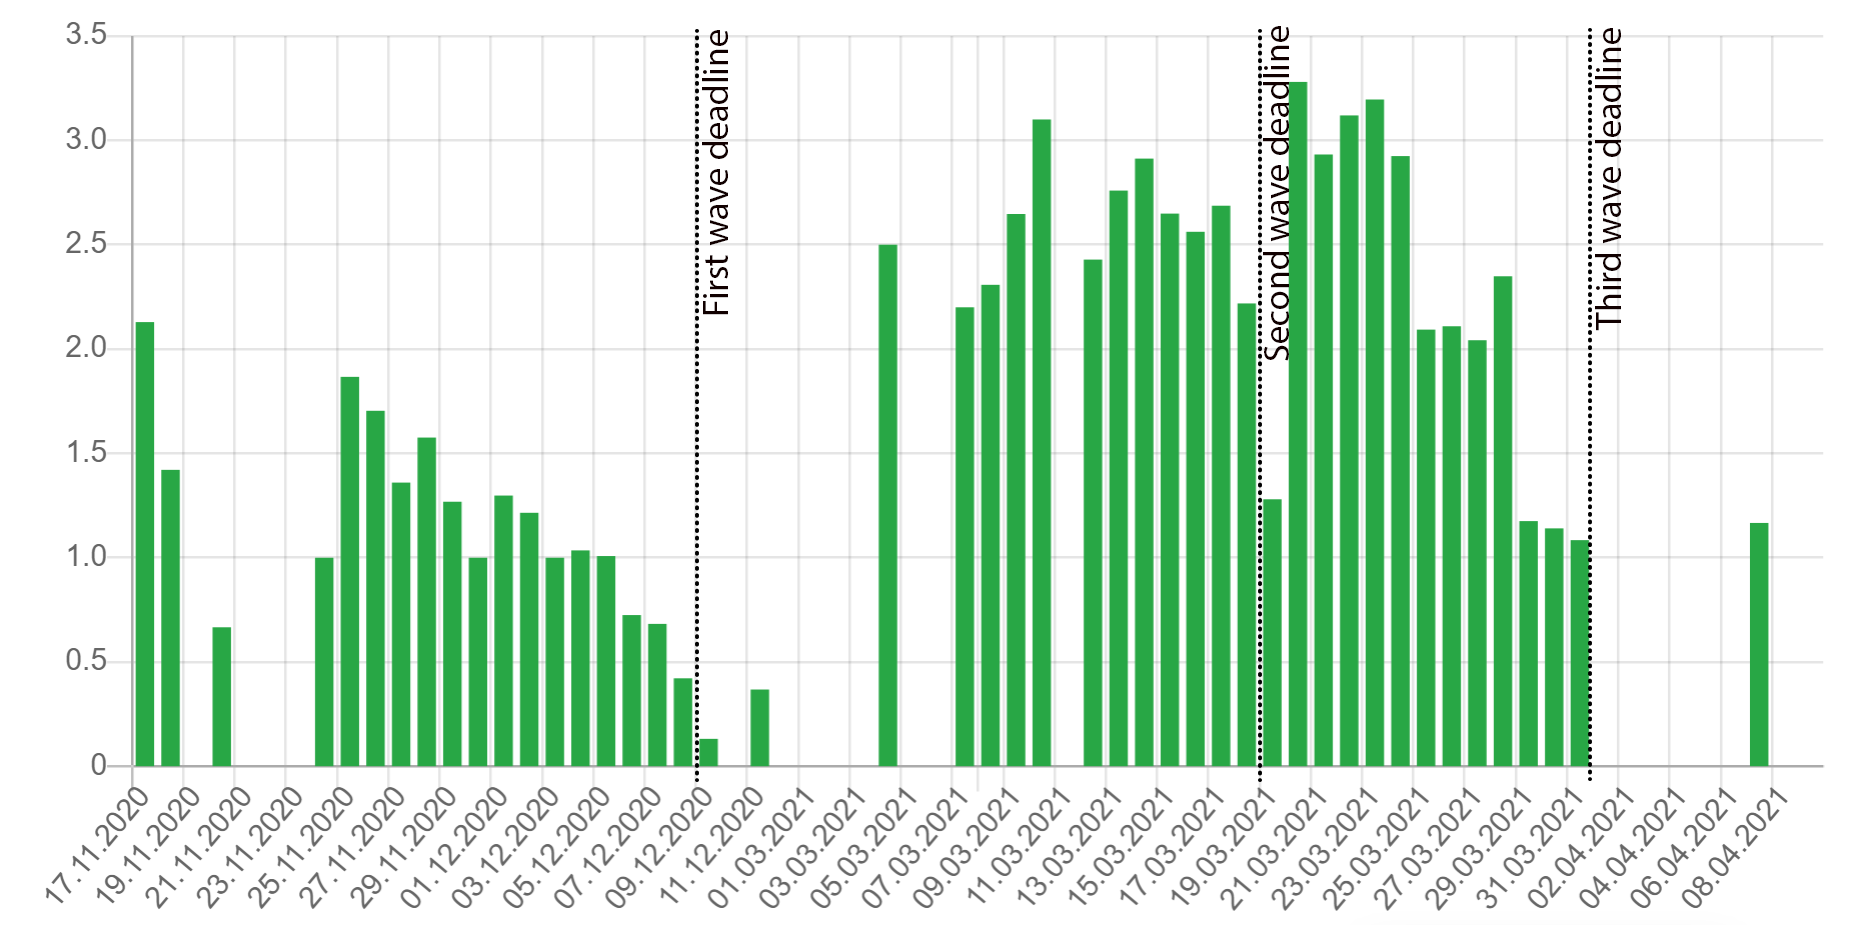
\includegraphics[width=18cm]{fig/number-of-crossannotations.png}}}
\caption[Average number of cross-annotations per claim by day]{Average number of cross-annotations per claim by day. Only counting annotations within the current wave (+2 days tolerance -- not showing the post-wave adjustments).}
\label{fig:crossannotations}
\end{figure} % zeleny graf

Due to the unbiased claim sampling in \tdvab{}, the late claims were extremely punished, as they were absent for most of its instances. The Figure~\ref{fig:crossannotations} shows this phenomenon -- on December $8^{th}$ the average number of annotations per claim descended below 0.5, which is very unfortunate, as the Figure~\ref{fig:performance} shows this day to be the second most productive in the claim mutation.

Therefore, we have biased the \tdva{} claim sampling in the following ways:
\begin{enumerate}
    \item $m^c$ is assigned a random priority from $(0,1)$
    \item If $m^c$ comes from the current wave of annotation, priority is incrementated by 1 
    \item If $m^c$ has less then 1 non-oracle annotation\footnote{Originally, we have tried to aim for 2 non-oracle annotations per claim, however, this was too punishing for the unannotated claims left from previous waves, as each new claim would be favoured for as long as it does not collect 2 annotations}, priority increments by 1
    \item Finally, $m^c$ with the highest priority is sent on output.
\end{enumerate}

Fast implementation of this sampling using the \textsf{SQL} \textit{subqueries} can be found in the attached  \texttt{LabelController.php}.

In addition to this, we have \textbf{adjusted the required number of data-points per task}.
From 5 \tjednaa{} claims, 15 \tjednab{} mutations, 5 \tdvaa{} oracle annotations and 15 \tdvab{} non-oracle annotations, we have switched to\textbf{ 3, 7, 7} and \textbf{35}, respectively (Figure~\ref{sec:workflow}), based on our stopwatch-per-task measurements and the findings from Figure~\ref{fig:crossannotations}, in which the $1^{st}$ \textit{Wave} partition shows the need for an increase in cross-annotations.

Lastly, we have dedicated the time to hand-annotate\textbf{ \char`~300 residual claims} after the last wave. These adjustments led to a significant improvement over the random baseline -- for instance, after the first wave deadline, around 40\% of all claims ended up with 0 annotations. By the time of the publication of this thesis, the amount of the 0-annotated claims decreased to only 9\%, still counting the original $1^{st}$ wave set, subject to its post-annotations.


\section{System Performance Remarks}
We have been surprised by the robustness and traffic resistance of the resulting scheme. Dataset does not contain traces of blackouts or \texttt{HTTP} communication interrupts between \textsf{Flask} and \textsf{Apache}. We also consider the traffic load carried by our system during the wave deadlines (Fig~\ref{fig:performance}) remarkable, given the size of the \textsf{ČTK Archive} and the complexity of the~\ref{sec:knowledge-scopes} algorithm. We attribute this to the full \textsf{AJAX}-initiated asynchronization of the costly operations and to the support we recieved from the \textsf{Faculty of Electrical Engineering}, namely Petr Benda, who provided us with a server with \textsf{Intel Xeon E3 CPU} and 132 GB of memory that runs both \textsf{Flask} and \textsf{Apache} apps to this date\footnote{As of May 20$^{th}$}.

\section{Annotation wrap-up}
We have successfully conducted three experiments on human annotation for the \textit{fact-checking using \textsf{ČTK Archive}} task, using a novel annotation platform of our own design, which is \textit{live} on \url{https://fcheck.fel.cvut.cz}, or can be installed from its source\footnote{\url{https://gitlab.fel.cvut.cz/factchecking/fcheck-anotations-platform}} that is to be published under a license to be specified in \texttt{LICENSE.md}.

We thank to all \textsf{FSS} students who participated in our experiments for donating their time to support our endeavours with a total of \textbf{4,325} valid \db{Claim}, and \textbf{5,759} \db{Label} datapoints.
According to their verbal feedback after the supplementary lectures, many of them enjoyed our cooperation\footnote{Even if, based on the textual inputs found in our database, at least one did not}, and the research partnership started with our project shall continue with other exciting future collaborations. 
